\section{Evaluation}
\label{sec:syn-eval}

We have implemented \toolName{} on top of the
Counter tool \cite{oopsla20}.
We use {\em four} SMT solvers running in parallel for solving
SMT proof obligations discharged by our proof discharge algorithm:
{\tt z3-4.8.7}, {\tt z3-4.8.14} \cite{z3},
{\tt Yices2-45e38fc} \cite{yices},
and {\tt cvc4-1.7} \cite{cvc4solver}.
An unroll factor of {\em four} is used to handle loop unrolling in the C implementation.
We use a default value of {\em eight} for
over- and under-approximation depths ($d_o$ and $d_u$).
The default value of
our unrolling parameter $k$ (used for categorization of proof obligations) is {\em five}.

\toolName{} requires the user to provide a \SpecL{} program (specification), a C implementation,
and a file that contains the precondition and postcondition. All inductive invariants
at intermediate nodes in the product-CFG are inferred automatically.
We consider programs involving four distinct ADTs, namely,
\inv{\small T1} \type{String}, \inv{\small T2} \type{List}, \inv{\small T3} \type{Tree}
and \inv{\small T4} \type{Matrix}.
% For example, the {\tt String} ADT is a sum-type formed by constructors
% {\tt Invalid} (to
% encode the well-formedness condition of a string, e.g., it should be non-null),
% {\tt Nil} (representing an empty string) and {\tt Cons} (representing
% a recursive construction formed through a product of a character byte and a string).

% For each C implementation, an equivalence check requires the identification of
% lifting constructors that relate C values to the ADT values in \SpecL{}.
% The relations between a \SpecL{} value and a lifted value derived from C values (and current memory state)
% may be required at the entry of both programs (i.e., in the precondition $Pre$),
% in the middle of both programs (i.e., in the inferred invariants at intermediate product-CFG
% nodes), and at the exit of both programs (i.e., in the postcondition $Post$).
% $Pre$ and $Post$ are user-specified, but the inductive invariants are inferred
% automatically by our algorithm.
% Our invariant inference algorithm derives
% the shape of the lifting constructors from the user-specified $Pre$ and $Post$,
% and uses these shapes in enumerating relational guesses at product-CFG nodes.
% The \recursiveRelations{} in the precondition,
% postcondition, and invariants may relate \SpecL{} ADT variables with the
% values lifted (through a lifting constructor) from C variables (and current
% memory state).

\begin{table}[t]
\caption{\label{tab:LiftingConsStr}String lifting constructors and their definitions.}
\vspace{-5px}
\begin{scriptsize}
\begin{center}
\begin{tabular}{|l|l|}
\hline
\multicolumn{1}{|c|}{\Tstrut \Bstrut\footnotesize Lifting Constructor} & \multicolumn{1}{c|}{\Tstrut \Bstrut \footnotesize Definition} \\
\hline
\hline
% \multicolumn{2}{|c|}{\Tstrut \Bstrut \inv{T1} {\tt List = LNil | LCons(i32, List)}} \\
% \hline
% $\mathrm{Clist^{u32[]}_m(p\ i\ n : i32)}$ & \makecell[l]{\Tstrut $\mathrm{\underline{if}\ (i\geq_{u}n)}$ $\mathrm{\underline{then}\ LNil}$ \\ \Bstrut $\mathrm{\underline{else}\ LCons(p[i]^m_{i32}, Clist^{u32[]}_m(p,i+1_{i32},n))}$} \\
% \hline
% $\mathrm{Clist^{lnode(u32)}_m(p:i32)}$ & \makecell[l]{\Tstrut $\mathrm{\underline{if}\ (p==0_{i32})}$ $\mathrm{\underline{then}\ LNil}$ \\ \Bstrut $\mathrm{\underline{else}\ LCons(\structPointer{\tt p}{m}{\tt lnode}{val}, Clist^{lnode}_m(\structPointer{\tt p}{m}{\tt lnode}{next})}$} \\
% \hline
% $\mathrm{Clist^{clnode(u32)}_m(p:i32,i:i2)}$ & \makecell[l]{\Tstrut $\mathrm{\underline{if}\ (p==0_{i32})}$ $\mathrm{\underline{then}\ LNil}$ \\ \Bstrut $\mathrm{\underline{else}\ LCons(\structPointer{\tt p}{m}{\tt clnode}{chunk}[i]^m_{i32}, Clist^{clnode}_m((ite(i==3_{i2}, \structPointer{\tt p}{m}{\tt clnode}{next},p), i+1_{i2}))}$} \\
% \hline
% $\mathrm{Clist^{u32[r]}_m(p\ i\ j\ u\ v:i32)}$ & \makecell[l]{\Tstrut $\mathrm{\underline{if}\ (j\geq_{u}v)}$ $\mathrm{\underline{then}\ LNil}$ \\ \Bstrut $\mathrm{\underline{else}\ LCons(p[i*v+j]^m_{i32}, Clist^{u32[r]}_m(p,i,j+1_{i32},u,v))}$} \\
% \hline
% $\mathrm{Clist^{u32[c]}_m(p\ i\ j\ u\ v:i32)}$ & \makecell[l]{\Tstrut $\mathrm{\underline{if}\ (j\geq_{u}v)}$ $\mathrm{\underline{then}\ LNil}$ \\ \Bstrut $\mathrm{\underline{else}\ LCons(p[i+j*u]^m_{i32}, Clist^{u32[c]}_m(p,i,j+1_{i32},u,v))}$} \\
% \hline
% \hline
% \multicolumn{2}{|c|}{\Tstrut \Bstrut \inv{T2} {\tt Tree = TNil | TCons(i32, Tree, Tree)}} \\
% \hline
% $\mathrm{Ctree^{u32[]}_m(p\ i\ n : i32)}$ & \makecell[l]{\Tstrut $\mathrm{\underline{if}\ (i \geq_{u} n)}$ $\mathrm{\underline{then}\ TNil}$ \\ \Bstrut $\mathrm{\underline{else}\ TCons(p[i]^{i32}_m, Ctree^{u32[]}_m(p,2_{i32}*i+1_{i32},n), Ctree^{u32[]}_m(p,2_{i32}*i+2_{i32},n))}$ } \\
% \hline
% $\mathrm{Ctree^{tnode(u32)}_m(p:i32)}$ & \makecell[l]{\Tstrut $\mathrm{\underline{if}\ (p==0_{i32})}$ $\mathrm{\underline{then}\ TNil}$ \\ \Bstrut $\mathrm{\underline{else}\ TCons(\structPointer{\tt p}{m}{\tt tnode}{val}, Ctree^{tnode}_m(\structPointer{\tt p}{m}{\tt tnode}{left}), Ctree^{tnode}_m(\structPointer{\tt p}{m}{\tt tnode}{right}))}$ } \\
% \hline
% \hline
\multicolumn{2}{|c|}{\Tstrut \Bstrut \inv{T1} {\tt Str = SInvalid | SNil | SCons(i8, Str)}} \\
\hline
$\mathrm{Cstr^{u8[]}_m(p:i32)}$ & \makecell[l]{\Tstrut $\mathrm{\underline{if}\ (p==0_{i32})}$ $\mathrm{\underline{then}\ SInvalid}$ \\ \Tstrut $\mathrm{\underline{else\ if}\ (p[0_{i32}]^m_{i8}==0_{i8})\ \underline{then}\ SNil}$ \\ \Bstrut $\mathrm{\underline{else}\ SCons(p[0_{i32}]^m_{i8}, Cstr^{u8[]}_m(p+1_{i32}))}$} \\
\hline
$\mathrm{Cstr^{lnode(u8)}_m(p:i32)}$ & \makecell[l]{\Tstrut $\mathrm{\underline{if}\ (p==0_{i32})}$ $\mathrm{\underline{then}\ SInvalid}$ \\ \Tstrut $\mathrm{\underline{else\ if}\ (\structPointer{\tt p}{m}{\tt lnode}{val} == 0_{i8})\ \underline{then}\ SNil}$ \\ \Bstrut $\mathrm{\underline{else}\ SCons(\structPointer{\tt p}{m}{\tt lnode}{val}, Cstr^{lnode(u8)}_m(\structPointer{\tt p}{m}{\tt lnode}{next}))}$} \\
\hline
$\mathrm{Cstr^{clnode(u8)}_m(p:i32,i:i2)}$ & \makecell[l]{\Tstrut $\mathrm{\underline{if}\ (p==0_{i32})}$ $\mathrm{\underline{then}\ SInvalid}$ \\ \Tstrut $\mathrm{\underline{else\ if}\ (\structPointer{\tt p}{m}{\tt clnode}{chunk} [i]^m_{i8} == 0_{i8})\ \underline{then}\ SNil}$ \\ \Bstrut $\mathrm{\underline{else}\ SCons(\structPointer{\tt p}{m}{\tt clnode}{chunk} [i]^m_{i8},}$ \\ \qquad \qquad \quad $\mathrm{Cstr^{clnode(u8)}_m((i==3_{i2}\ ?\ \structPointer{\tt p}{m}{\tt clnode}{next}\ :\ p), i+1_{i2}))}$} \\
\hline
% \hline
% \multicolumn{2}{|c|}{\Tstrut \Bstrut \inv{T4} {\tt Matrix = MNil | MCons(List, Matrix)}} \\
% \hline
% $\mathrm{Cmat^{u32[][]}_m(p\ i\ u\ v:i32)}$ & \makecell[l]{\Tstrut $\mathrm{\underline{if}\ (i \geq_{u} u)}$ $\mathrm{\underline{then}\ MNil}$ \\ \Bstrut $\mathrm{\underline{else}\ MCons(Clist^{u32[]}_m(p[i]^m_{i32},0_{i32},v), Cmat^{u32[][]}_m(p,i+1_{i32},u,v))}$} \\
% \hline
% $\mathrm{Cmat^{u32[r]}_m(p\ i\ u\ v:i32)}$ & \makecell[l]{\Tstrut $\mathrm{\underline{if}\ (i \geq_{u} u)}$ $\mathrm{\underline{then}\ MNil}$ \\ \Bstrut $\mathrm{\underline{else}\ MCons(Clist^{u32[r]}_m(p,i,0_{i32},u,v), Cmat^{u32[r]}_m(p,i+1_{i32},u,v))}$} \\
% \hline
% $\mathrm{Cmat^{u32[c]}_m(p\ i\ u\ v:i32)}$ & \makecell[l]{\Tstrut $\mathrm{\underline{if}\ (i \geq_{u} u)}$ $\mathrm{\underline{then}\ MNil}$ \\ \Bstrut $\mathrm{\underline{else}\ MCons(Clist^{u32[c]}_m(p,i,0_{i32},u,v), Cmat^{u32[c]}_m(p,i+1_{i32},u,v))}$} \\
% \hline
% $\mathrm{Cmat^{lnode(u32[])}_m(p\ v:i32)}$ & \makecell[l]{\Tstrut $\mathrm{\underline{if}\ (p==0_{i32})}$ $\mathrm{\underline{then}\ MNil}$ \\ \Bstrut $\mathrm{\underline{else}\ MCons(Clist^{u32[]}_m(\structPointer{\tt p}{m}{\tt lnode}{val},0_{i32},v),Cmat^{lnode(u32[])}_m(\structPointer{\tt p}{m}{\tt lnode}{next},v))}$} \\
% \hline
% $\mathrm{Cmat^{lnode(u32)[]}_m(p\ i\ u:i32)}$ & \makecell[l]{\Tstrut $\mathrm{\underline{if}\ (i \geq u)}$ $\mathrm{\underline{then}\ MNil}$ \\ \Bstrut $\mathrm{\underline{else}\ MCons(Clist^{lnode(u32)}_m(p[i]^m_{i32}), Cmat^{lnode(u32)[]}_m(p,i+1_{i32},u))}$} \\
% \hline
% $\mathrm{Cmat^{clnode(u32)[]}_m(p\ i\ u:i32)}$ & \makecell[l]{\Tstrut $\mathrm{\underline{if}\ (i \geq u)}$ $\mathrm{\underline{then}\ MNil}$ \\ \Bstrut $\mathrm{\underline{else}\ MCons(Clist^{clnode(u32)}_m(p[i]^m_{i32},0_{i2}), Cmat^{clnode(u32)[]}_m(p,i+1_{i32},u))}$} \\
% \hline
\end{tabular}
\end{center}
\end{scriptsize}
\end{table}

\subsection{Experiments}
For each \SpecL{} program specification, we consider multiple
C implementations that differ in their (a) layout and representation of ADTs, and
(b) algorithmic strategies. For example, a \type{Matrix}, in C, may be laid out
in a two-dimensional array, a one-dimensional array using row or column major
layouts etc. On the other hand, an optimized implementation may choose manual vectorization
of an inner-most loop. Next, we consider each ADT in more detail. For each,
we discuss (a) its corresponding programs, (b) C memory layouts and their lifting
constructors, and (c) varying algorithmic strategies.

% The required lifting constructor may be different for different data layouts.
% \Cref{tab:LiftingConsTable} shows the various lifting constructors used for validating
% the benchmarks we describe below. In this table,
% we use {\tt lnode(T)} to represent a linked list node
% which encapsulates a value of type {\tt T}.
% Similarly, {\tt clnode(T)} and {\tt tnode(T)} represent
% a chunked linked list node and a tree node respectively
% that encapsulate
% value(s) of type {\tt T}. {\tt u32} represents
% the 32-bit unsigned integer type.
% We use a ternary {\tt ite(c,x,y)} operator which
% returns {\tt x} if {\tt c} evaluates to true and {\tt y} otherwise.
% The syntax {\tt T[]} represents an array of type {\tt T}.
% {\tt T[r]} and {\tt T[c]} represent flattened
% arrays of type {\tt T}, flattened using row-major and column-major
% formats respectively.

\begin{figure}
\begin{subfigure}[b]{0.5\textwidth}
\begin{center}
\begin{allLangEnvFoot}
~{\tiny \textcolor{mygray}{S0:}}~ i32 strlen (Str s) {
~{\tiny \textcolor{mygray}{S1:}}~   i32 len $\coloneqq$ ${\tt 0_{i32}}$;
~{\tiny \textcolor{mygray}{S2:}}~   while $\neg$(s is SNil):
~{\tiny \textcolor{mygray}{S3:}}~     assume $\neg$(s is SInvalid);
~{\tiny \textcolor{mygray}{S4:}}~     // (s is SCons)
~{\tiny \textcolor{mygray}{S5:}}~     s   $\coloneqq$ s.tail;
~{\tiny \textcolor{mygray}{S6:}}~     len $\coloneqq$ len + ${\tt 1_{i32}}$;
~{\tiny \textcolor{mygray}{S7:}}~   return len;
~{\tiny \textcolor{mygray}{SE:}}~ }
\end{allLangEnvFoot}
\end{center}
\caption{\label{fig:llStrlenSpecIR}Strlen specification}
\end{subfigure}%
\begin{subfigure}[b]{0.5\textwidth}
\begin{center}
\vspace{5px}
\begin{allLangEnvFoot}
~{\tiny \textcolor{mygray}{\ \ \ }}~ size_t strlen(char* s);

~{\tiny \textcolor{mygray}{C0:}}~ i32 strlen (i32 s) {
~{\tiny \textcolor{mygray}{C1:}}~   i32 i $\coloneqq$ ${\tt 0_{i32}}$;
~{\tiny \textcolor{mygray}{C2:}}~   while $\arrIndex{\tt s}{0_{i32}}{\mem{}}{i8} \neq 0_{i8}$:
~{\tiny \textcolor{mygray}{C3:}}~     s $\coloneqq$ s + ${\tt 1_{i32}}$;
~{\tiny \textcolor{mygray}{C4:}}~     i $\coloneqq$ i + ${\tt 1_{i32}}$;
~{\tiny \textcolor{mygray}{C5:}}~   return i;
~{\tiny \textcolor{mygray}{CE:}}~ }
\end{allLangEnvFoot}
\end{center}
\caption{\label{fig:llStrlenCArrIR}Generic strlen implementation using array}
\end{subfigure}
\begin{subfigure}[b]{1\textwidth}
\begin{center}
\begin{allLangEnvFoot}
~{\tiny \textcolor{mygray}{\ \ \ \ }}~ typedef struct clnode {
~{\tiny \textcolor{mygray}{\ \ \ \ }}~   char chunk[4]; struct clnode* next; } clnode;
~{\tiny \textcolor{mygray}{\ \ \ \ }}~ size_t strlen(clnode* cl);

~{\tiny \textcolor{mygray}{C0:\phantom{ }}}~ i32 strlen (i32 cl) {
~{\tiny \textcolor{mygray}{C1:\phantom{ }}}~   i32 hi $\coloneqq$ ${\tt 0x80808080_{i32}}$; i32 lo $\coloneqq$ ${\tt 0x01010101_{i32}}$;
~{\tiny \textcolor{mygray}{C2:\phantom{ }}}~   i32 i  $\coloneqq$ ${\tt 0_{i32}}$;
~{\tiny \textcolor{mygray}{C3:\phantom{ }}}~   while ${\tt true}$:
~{\tiny \textcolor{mygray}{C4:\phantom{ }}}~     i32 dword_ptr $\coloneqq$ addrof($\structPointer{\tt cl}{\mem{}}{clnode}{chunk}$);
~{\tiny \textcolor{mygray}{C5:\phantom{ }}}~     i32 dword     $\coloneqq$ $\arrIndex{\tt dword\_ptr}{0_{i32}}{\mem{}}{i32}$;
~{\tiny \textcolor{mygray}{C6:\phantom{ }}}~     if ${\tt ((dword - lo)\ \&\ (\sim dword)\ \&\ hi) \neq 0_{i32}}$:
~{\tiny \textcolor{mygray}{C7:\phantom{ }}}~       if $\arrIndex{\tt dword\_ptr}{0_{i32}}{\mem{}}{i8} = 0_{i8}$: return i;
~{\tiny \textcolor{mygray}{C8:\phantom{ }}}~       if $\arrIndex{\tt dword\_ptr}{1_{i32}}{\mem{}}{i8} = 0_{i8}$: return ${\tt i + 1_{i32}}$;
~{\tiny \textcolor{mygray}{C9:\phantom{ }}}~       if $\arrIndex{\tt dword\_ptr}{2_{i32}}{\mem{}}{i8} = 0_{i8}$: return ${\tt i + 2_{i32}}$;
~{\tiny \textcolor{mygray}{C10:}}~       if $\arrIndex{\tt dword\_ptr}{3_{i32}}{\mem{}}{i8} = 0_{i8}$: return ${\tt i + 3_{i32}}$;
~{\tiny \textcolor{mygray}{C11:}}~     cl $\coloneqq$ $\structPointer{\tt cl}{\mem{}}{clnode}{next}$; i  $\coloneqq$ ${\tt i + 4_{i32}}$;
~{\tiny \textcolor{mygray}{CE:\phantom{ }}}~ }
\end{allLangEnvFoot}
\end{center}
\caption{\label{fig:llStrlenCClistIR}Optimized strlen implementation using chunked linked list}
\end{subfigure}%
\caption{\label{fig:strlenSpecAndC}\Cref{fig:llStrlenSpecIR} shows the (abstracted) IR for the \SpecL{} specification of {\tt strlen}.
\Cref{fig:llStrlenCArrIR,fig:llStrlenCClistIR} show the (abstracted) IRs for two C implementations of {\tt strlen}.
\Cref{fig:llStrlenCArrIR} is a generic implementation using a nul-terminated array to represent a string, whereas
\cref{fig:llStrlenCClistIR} is an optimized implementation with a chunked linked list memory layout for a string.}
\end{figure}


\subsubsection{String} We wrote a single specification in \SpecL{} for each of the
following
common string library functions: {\tt strlen}, {\tt strchr}, {\tt strcmp}, {\tt strspn},
{\tt strcspn}, and {\tt strpbrk}.  For each specification
program, we took multiple C implementations of that program, drawn from popular
libraries like {\tt glibc} \cite{glibc}, {\tt klibc} \cite{klibc}, {\tt newlib} \cite{newlib},
{\tt openbsd} \cite{openbsdlibc}, {\tt uClibc} \cite{uclibc},
{\tt dietlibc} \cite{dietlibc}, {\tt musl} \cite{musl}, and {\tt netbsd} \cite{netbsd}.
Some of these libraries implement the same function in two ways: one that is optimized
for code size (subscripted with $s$) and another that is optimized for runtime (subscripted with $f$).
All these library implementations use a {\em null character} terminated array to represent
a string, and the
corresponding lifting constructor is \lift{str}{\mem{}}{u8[]}.
\type{u<N>} represents the N-bit unsigned integer type in C.
For example, \type{u8} represents \type{unsigned char} type.

Further, we implemented
custom C programs for all of these functions that used
linked list
and {\em chunked linked list} data structures
to represent a string.
In a chunked linked list, a single list node (linked
through a {\tt next} pointer)
contains a small array (chunk) of values.
We use a default chunk size of four for our
benchmarks.
The corresponding lifting constructors are \lift{str}{\mem{}}{lnode(u8)}
and \lift{str}{\mem{}}{clnode(u8)} respectively.
These lifting constructors are defined in \cref{tab:LiftingConsStr}.
\lift{str}{\mem{}}{lnode(u8)} requires a single
argument $p$ representing the pointer to the list node.
On the other hand, \lift{str}{\mem{}}{clnode(u8)} requires two arguments $p$
and $i$, where $p$ represents the pointer to the chunked linked list node
and $i$ represents the position of the initial character in the chunk.

Usually, we name a lifting constructor based on its underlying data layout.
For example, \lift{str}{\mem{}}{lnode(u8)} represents a lifting constructor
for a chunked linked list of characters as its underlying data layout.
In general, we use the following naming convension for different data layouts.
\type{T[]} represents an array of type \type{T} (e.g., \type{u8[]}).
\type{lnode(T)} represents a  linked list node type which encapsulates a value of type \type{T}.
Similarly, \type{clnode(T)} and \type{tnode(T)} represent a chunked linked list and a tree node
containing values of type \type{T} respectively.

\begin{figure}[t!]
\begin{tabular}{@{}c@{}c@{}}
\begin{subfigure}[b]{0.50\textwidth}
\begin{center}
{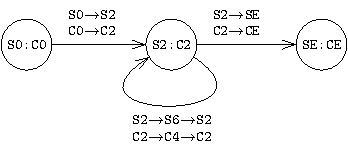
\includegraphics[scale=1.2]{chapters/figures/figStrlenArrProductCfg.pdf}}
\end{center}
\caption{\label{fig:StrlenArrProductCFG}Product-CFG for programs \cref{fig:llStrlenSpecIR,fig:llStrlenCArrIR}}
\end{subfigure}%
&
\begin{subfigure}[b]{0.50\textwidth}
\begin{center}
\begin{scriptsize}
\begin{tabular}{cl}
\toprule
{\bf PC-Pair} & \multicolumn{1}{c} {\bf Invariants} \\
\toprule
(\scpc{0}{0}) &
\Tstrut $\circled{P}\ \sv{s} \indEq{} \lifted{str}{\mem{}}{char[]}{\cv{s}}$ \\
\midrule
\multirow{2}{*}{(\scpc{2}{2})} &
\Tstrut $\circled{\tiny I1} \ \sv{s} \indEq{} \lifted{str}{\mem{}}{char[]}{\cv{s}}$ \\ &
\Tstrut $\circled{\tiny I2} \ \sv{len} = \cv{i}$ \\
\midrule
(\scpc{E}{E}) &
\Tstrut \Bstrut $\circled{E}\ \sv{ret} = \cv{ret}$ \\
\bottomrule
\end{tabular}
\end{scriptsize}
\end{center}
\caption{\label{fig:StrlenArrInvs}Invariants for product-CFG in \cref{fig:StrlenArrProductCFG}}
\end{subfigure}%
\\
\begin{subfigure}[b]{0.50\textwidth}
\begin{center}
{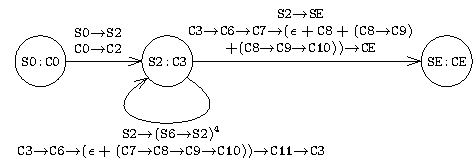
\includegraphics[scale=1.15]{chapters/figures/figStrlenClProductCfg.pdf}}
\end{center}
\caption{\label{fig:StrlenClProductCFG}Product-CFG for programs \cref{fig:llStrlenSpecIR,fig:llStrlenCClistIR}}
\end{subfigure}%
&
\begin{subfigure}[b]{0.50\textwidth}
\begin{center}
\begin{scriptsize}
\begin{tabular}{cl}
\toprule
{\bf PC-Pair} & \multicolumn{1}{c} {\bf Invariants} \\
\toprule
(\scpc{0}{0}) &
\Tstrut $\circled{P}\ \sv{s} \indEq{} \lifted{str}{\mem{}}{clnode}{\cv{cl},0}$ \\
\midrule
\multirow{2}{*}{(\scpc{2}{3})} &
\Tstrut $\circled{\tiny I1} \ \sv{s} \indEq{} \lifted{str}{\mem{}}{clnode}{\cv{cl},0}$ \\ &
\Tstrut $\circled{\tiny I2} \ \sv{len} = \cv{i}$ \\
\midrule
(\scpc{E}{E}) &
\Tstrut \Bstrut $\circled{E} \ \sv{ret} = \cv{ret}$ \\
\bottomrule
\end{tabular}
\end{scriptsize}
\end{center}
\caption{\label{fig:StrlenClInvs}Invariants for product-CFG in \cref{fig:StrlenClProductCFG}}
\end{subfigure}%
\end{tabular}
\caption{\label{fig:StrlenProductCFGsAndInvs}Product-CFGs and their node invariants representing bisimulation relations between the specification \cref{fig:llStrlenSpecIR}
and its two implementations in \cref{fig:llStrlenCArrIR,fig:llStrlenCClistIR} respectively.}
\end{figure}

\Cref{fig:strlenSpecAndC} shows the {\tt strlen} specification and two vastly
different $C$ implementations. \Cref{fig:llStrlenCArrIR} is a generic implementation
using a null character terminated array to represent a string similar to a C-style string.
The second implementation in \cref{fig:llStrlenCClistIR} differs from \cref{fig:llStrlenCArrIR}
in the following: (a) it uses a chunked linked list data layout for the input string
and (b) it uses specialized bit manipulations to identify a null character in a chunk at a time.
\toolName{} is able to automatically find a bisimulation relation showing equivalence
for both implementations against the unaltered specification.
\Cref{fig:StrlenProductCFGsAndInvs} shows the product-CFG and invariants for each implementation.

\begin{center}
\begin{table}[H]
\begin{scriptsize}
\begin{tabular}{|l|l|}
\hline
\multicolumn{1}{|c|}{\Tstrut \Bstrut\footnotesize Lifting Constructor} & \multicolumn{1}{c|}{\Tstrut \Bstrut \footnotesize Definition} \\
\hline
\hline
\multicolumn{2}{|c|}{\Tstrut \Bstrut \inv{T1} {\tt Str = SInvalid | SNil | SCons(ch:i8, tail:Str)}} \\
\hline
$\mathrm{Cstr^{char[]}_m(p:i32)}$ & \makecell[l]{\Tstrut $\mathrm{\underline{if}\ (p==0_{i32})}$ $\mathrm{\underline{then}\ SInvalid}$ \\ \Tstrut $\mathrm{\underline{else\ if}\ (p[0_{i32}]^m_{i8}==0_{i8})\ \underline{then}\ SNil}$ \\ \Bstrut $\mathrm{\underline{else}\ SCons(p[0_{i32}]^m_{i8}, Cstr^{char[]}_m(p+1_{i32}))}$} \\
\hline
$\mathrm{Cstr^{lnode(char)}_m(p:i32)}$ & \makecell[l]{\Tstrut $\mathrm{\underline{if}\ (p==0_{i32})}$ $\mathrm{\underline{then}\ SInvalid}$ \\ \Tstrut $\mathrm{\underline{else\ if}\ (\structPointer{\tt p}{m}{\tt lnode}{val} == 0_{i8})\ \underline{then}\ SNil}$ \\ \Bstrut $\mathrm{\underline{else}\ SCons(\structPointer{\tt p}{m}{\tt lnode}{val}, Cstr^{lnode}_m(\structPointer{\tt p}{m}{\tt lnode}{next}))}$} \\
\hline
$\mathrm{Cstr^{clnode(char)}_m(p:i32,i:i2)}$ & \makecell[l]{\Tstrut $\mathrm{\underline{if}\ (p==0_{i32})}$ $\mathrm{\underline{then}\ SInvalid}$ \\ \Tstrut $\mathrm{\underline{else\ if}\ (\structPointer{\tt p}{m}{\tt clnode}{chunk} [i]^m_{i8} == 0_{i8})\ \underline{then}\ SNil}$ \\ \Bstrut $\mathrm{\underline{else}\ SCons(\structPointer{\tt p}{m}{\tt clnode}{chunk} [i]^m_{i8},}$ \\ \qquad \qquad \quad $\mathrm{Cstr^{clnode}_m((ite(i==3_{i2},\structPointer{\tt p}{m}{\tt clnode}{next} , p), i+1_{i2}))}$} \\
\hline
\end{tabular}
\end{scriptsize}
\caption{\label{tab:LiftingConsStr}Lifting constructors and their definitions for {\tt String} ADT.}
\vspace{-18px}
\end{table}
\end{center}

\vspace{-10px}
\subsubsection{List} We wrote a \SpecL{} program specification that creates a list, a
program that traverses a list to compute the sum of its elements and a program
that computes the dot product of two lists. We use three different
data layouts for a list in C: character array (\lift{list}{\mem{}}{u32[]}),
linked list (\lift{list}{\mem{}}{lnode(u32)}), and
a chunked linked list (\lift{list}{\mem{}}{clnode(u32)}).
The lifting constructors are shown in \cref{tab:LiftingConsList}.
Although similar to the String lifting constructors, these lifting
constructors differ widely in their data encodings. For example,
\lifted{list}{\mem{}}{u32[]}{p,i,n} represents a \type{List} value constructed
from a C array $p$ of size $n$ starting at the $i^{th}$ index. The list becomes empty
when we are at the end of the array. (\lift{list}{\mem{}}{lnode(u32)})
and (\lift{list}{\mem{}}{clnode(u32)}), on the other hand, encodes empty
lists (\cons{LNil}) using {\em null pointers}. These encodings are in contrast to the
\type{String} lifting constructors, all of which uses a {\em null character} to
encode the empty string.

\begin{table}[H]
\begin{center}
\caption{\label{tab:LiftingConsTree}Tree lifting constructors and their definitions.}
\begin{scriptsize}
\begin{tabular}{|l|l|}
\hline
\multicolumn{1}{|c|}{\Tstrut \Bstrut\footnotesize \bf Lifting Constructor} & \multicolumn{1}{c|}{\Tstrut \Bstrut \footnotesize \bf Definition} \\
\hline
\hline
\multicolumn{2}{|c|}{\Tstrut \Bstrut \inv{T3} {\tt Tree = TNil | TCons(i32, Tree, Tree)}} \\
\hline
\lifted{tree}{\mem{}}{u32[]}{p\ i\ n\ctype{i32}} & \makecell[l]{\Tstrut \sumIf{i \geq_u n} \  \sumThen{\cons{TNil}} \\
                                                        \Tstrut \Bstrut \sumElse{\cons{TCons}(\arrIndex{p}{i}{i32}{\mem{}}, \lifted{tree}{\mem{}}{u32[]}{p,2_\type{i32} \times i+1_\type{i32},n}, \lifted{tree}{\mem{}}{u32[]}{p,2_\type{i32} \times i+2_\type{i32},n})}} \\
\hline
\lifted{tree}{\mem{}}{tnode(u32)}{p\ctype{i32}} & \makecell[l]{\Tstrut \sumIf{p = 0_\type{i32}} \  \sumThen{\cons{TNil}} \\
                                                       \Tstrut \Bstrut \sumElse{\cons{TCons}(\structPointer{p\!}{\mem{}}{tnode}{\!\!val},\! \lifted{tree}{\mem{}}{tnode(u32)}{\structPointer{p\!}{\mem{}}{tnode}{\!\!left}},\! \lifted{tree}{\mem{}}{tnode(u32)}{\structPointer{p\!}{\mem{}}{tnode}{\!\!right}})}} \\
\hline
\end{tabular}
\end{scriptsize}
\end{center}
\end{table}
\vspace{-10px}
\subsubsection{Tree} We wrote a \SpecL{} program that sums all the nodes in a tree
through an inorder traversal using recursion. We use two different data layouts for a tree: 
(1) a flat array where a
complete binary tree is laid out in breadth-first search order commonly used for heaps (\lift{tree}{\mem{}}{u32[]}),
and (2) a linked tree node with two pointers for the left and right children (\lift{tree}{\mem{}}{tnode(u32)}).
Both \SpecL{} and C programs contain non-tail recursive procedure calls for left and right children.
\toolName{} is able to correlate these recursive calls using user-provided $Pre$ and $Post$.
At the entry of the recursive calls, \toolName{} is required to prove that $Pre$ holds for the arguments
and at the exit of the recursive calls, \toolName{} assumes $Post$ on the returned states.

\begin{table}[H]
\caption{\label{tab:LiftingConsMatrix}Matrix and auxiliary lifting constructors and their definitions.}
\vspace{-10px}
\begin{scriptsize}
\begin{center}
\begin{tabular}{|l|l|}
\hline
\multicolumn{1}{|c|}{\Tstrut \Bstrut\footnotesize Lifting Constructor} & \multicolumn{1}{c|}{\Tstrut \Bstrut \footnotesize Definition} \\
\hline
\hline
\multicolumn{2}{|c|}{\Tstrut \Bstrut \inv{T4} {\tt Matrix = MNil | MCons(List, Matrix)}} \\
\hline
$\mathrm{Cmat^{u32[][]}_m(p\ i\ u\ v:i32)}$ & \makecell[l]{\Tstrut $\mathrm{\underline{if}\ (i \geq_{u} u)}$ $\mathrm{\underline{then}\ MNil}$ \\ \Bstrut $\mathrm{\underline{else}\ MCons(Clist^{u32[]}_m(p[i]^m_{i32},0_{i32},v), Cmat^{u32[][]}_m(p,i+1_{i32},u,v))}$} \\
\hline
\hline
$\mathrm{Clist^{u32[r]}_m(p\ i\ j\ u\ v:i32)}$ & \makecell[l]{\Tstrut $\mathrm{\underline{if}\ (j\geq_{u}v)}$ $\mathrm{\underline{then}\ LNil}$ \\ \Bstrut $\mathrm{\underline{else}\ LCons(p[i*v+j]^m_{i32}, Clist^{u32[r]}_m(p,i,j+1_{i32},u,v))}$} \\
\hline
$\mathrm{Cmat^{u32[r]}_m(p\ i\ u\ v:i32)}$ & \makecell[l]{\Tstrut $\mathrm{\underline{if}\ (i \geq_{u} u)}$ $\mathrm{\underline{then}\ MNil}$ \\ \Bstrut $\mathrm{\underline{else}\ MCons(Clist^{u32[r]}_m(p,i,0_{i32},u,v), Cmat^{u32[r]}_m(p,i+1_{i32},u,v))}$} \\
\hline
\hline
$\mathrm{Clist^{u32[c]}_m(p\ i\ j\ u\ v:i32)}$ & \makecell[l]{\Tstrut $\mathrm{\underline{if}\ (j\geq_{u}v)}$ $\mathrm{\underline{then}\ LNil}$ \\ \Bstrut $\mathrm{\underline{else}\ LCons(p[i+j*u]^m_{i32}, Clist^{u32[c]}_m(p,i,j+1_{i32},u,v))}$} \\
\hline
$\mathrm{Cmat^{u32[c]}_m(p\ i\ u\ v:i32)}$ & \makecell[l]{\Tstrut $\mathrm{\underline{if}\ (i \geq_{u} u)}$ $\mathrm{\underline{then}\ MNil}$ \\ \Bstrut $\mathrm{\underline{else}\ MCons(Clist^{u32[c]}_m(p,i,0_{i32},u,v), Cmat^{u32[c]}_m(p,i+1_{i32},u,v))}$} \\
\hline
\hline
$\mathrm{Cmat^{lnode(u32[])}_m(p\ v:i32)}$ & \makecell[l]{\Tstrut $\mathrm{\underline{if}\ (p==0_{i32})}$ $\mathrm{\underline{then}\ MNil}$ \\ \Bstrut $\mathrm{\underline{else}\ MCons(Clist^{u32[]}_m(\structPointer{\tt p}{m}{\tt lnode}{val},0_{i32},v),}$ \\ \qquad\qquad\ \ \ \  $\mathrm{Cmat^{lnode(u32[])}_m(\structPointer{\tt p}{m}{\tt lnode}{next},v))}$} \\
\hline
$\mathrm{Cmat^{lnode(u32)[]}_m(p\ i\ u:i32)}$ & \makecell[l]{\Tstrut $\mathrm{\underline{if}\ (i \geq u)}$ $\mathrm{\underline{then}\ MNil}$ \\ \Bstrut $\mathrm{\underline{else}\ MCons(Clist^{lnode(u32)}_m(p[i]^m_{i32}),}$ \\ \qquad\qquad\ \ \ \  $\mathrm{Cmat^{lnode(u32)[]}_m(p,i+1_{i32},u))}$} \\
\hline
$\mathrm{Cmat^{clnode(u32)[]}_m(p\ i\ u:i32)}$ & \makecell[l]{\Tstrut $\mathrm{\underline{if}\ (i \geq u)}$ $\mathrm{\underline{then}\ MNil}$ \\ \Bstrut $\mathrm{\underline{else}\ MCons(Clist^{clnode(u32)}_m(p[i]^m_{i32},0_{i2}),}$ \\ \qquad\qquad\ \ \ \  $\mathrm{Cmat^{clnode(u32)[]}_m(p,i+1_{i32},u))}$} \\
\hline
\end{tabular}
\end{center}
\end{scriptsize}
\end{table}

\vspace{-10px}
\subsubsection{Matrix} We wrote a
\SpecL{} program to count the frequency of a value appearing in a 2D matrix.
A matrix is represented as an ADT that resembles a \type{List} of \type{List}s (\inv{\small T4} in \cref{tab:LiftingConsMatrix}).
The C implementations for a \type{Matrix} object include
(a) a two-dimensional array (\lift{mat}{\mem{}}{u32[][]}), (b) a flattened row-major array (\lift{mat}{\mem{}}{u32[r]}),
(c) a flattened column-major array (\lift{mat}{\mem{}}{u32[c]}), (d) a linked list of 1D arrays (\lift{mat}{\mem{}}{lnode(u32[])}),
(e) a 1D array of linked lists (\lift{mat}{\mem{}}{lnode(u32)[]}) and (f) a 1D array of chunked linked list (\lift{mat}{\mem{}}{clnode(u32)[]})
data layouts. Note that both \type{T[r]} and \type{T[c]} represent a 1D array of type {\tt T}. The {\em r} and {\em c} simply
emphasizes that these arrays are used to represent matrices in row-major and column-major encodings respectively.
We also introduce two auxiliary lifting constructors, \lift{list}{\mem{}}{u32[r]} and \lift{list}{\mem{}}{u32[c]}
for lifting each row of matrices lifted using the corresponding \lift{mat}{\mem{}}{u32[r]} and \lift{mat}{\mem{}}{u32[c]} \type{Matrix} lifting
constructors. These constructors are listed in \cref{tab:LiftingConsMatrix}.

\begin{figure}[H]
\begin{scriptsize}
\begin{tabular}{lllclllc}
\toprule
{\bf Data Layout} & {\bf Variant} & {\bf Time(s)} & {\bf ${\tt \bf ( d_u, d_o )}$} & {\bf Data Layout} & {\bf Variant} & {\bf Time(s)} & {\bf ${\tt \bf ( d_u, d_o )}$} \\
\midrule
\multicolumn{4}{c}{\bf list} &                                              \multicolumn{4}{c}{\bf tree} \\
u32[] & sum naive & 16 & (1,2) &                                           u32[] & sum & 264 & (1,2) \\
      & sum opt & 49 & (4,5) &                                             tnode(u32) & sum & 204 & (1,2) \\
lnode(u32) & sum naive & 8 & (1,2) &                                      \multicolumn{4}{c}{\bf matfreq} \\             
           & sum opt & 54 & (4,5) &                                       char[][] & naive & 974 & (1,3) \\                                      
           & create & 426 & (1,1) &                                                & opt & 1.8k & (4,8) \\                                       
clnode(u32) & sum opt & 39 & (4,5) &                                      char[r] & naive & 958 & (1,3) \\                                       
\multicolumn{4}{c}{\bf strlen}   &                                            & opt & 1.9k & (4,8) \\                                        
char[] & dietlibc$\mathrm{_{small}}$ & 9 & (1,2) &                             char[c] & naive & 984 & (1,3) \\                                       
       & dietlibc$\mathrm{_{fast}}$ & 44 & (3,2) &                                     & opt & 1.9k & (4,6) \\
       & glibc & 52 & (3,2) &                                                  lnode(char[]) & naive & 753 & (1,3) \\
       & klibc & 9 & (1,2) &                                                         & opt & 1.7k & (4,6) \\ 
       & musl & 49 & (3,2) &                                                   lnode(char)[] & naive & 1.5k & (1,2) \\
       & netbsd & 9 & (1,2) &                                                                & opt & 2.3k & (4,6) \\
       & newlib & 50 & (3,2) &                                              clnode(char)[] & opt & 1.8k & (4,6) \\
       & openbsd & 8 & (1,2) &                                                \multicolumn{4}{c}{\bf strpbrk} \\ 
       & uClibc & 8 & (1,2) &                                                 char[], char[] & dietlibc & 398 & (1,2) \\
lnode(char) & naive & 13 & (1,2) &                                                          & opt      & 494 & (4,2) \\
            & opt & 49 & (3,5) &                                              char[], lnode(char) & naive & 392 & (1,2) \\
clnode(char) & opt & 45 & (3,5) &                                                                & opt & 540 & (4,2) \\ 
 \multicolumn{4}{c}{\bf strchr} &                                                 char[], clnode(char) & opt & 523 & (4,2) \\
char[] & dietlibc$\mathrm{_{small}}$ & 16 & (1,1) &                           lnode(char), char[] & naive & 497 & (1,2) \\
       & dietlibc$\mathrm{_{fast}}$ & 89 & (4,1) &                                               & opt & 602 & (4,2) \\ 
       & glibc & 127 & (4,1) &                                                lnode(char), lnode(char) & naive & 345 & (1,2) \\
       & klibc & 23 & (1,1) &                                                                           & opt & 503 & (4,2) \\
       & newlib$\mathrm{_{small}}$ & 15 & (1,1) &                         lnode(char), clnode(char) & opt & 572 & (4,2) \\
       & openbsd & 24 & (1,1) &                                             \multicolumn{4}{c}{\bf strcspn} \\
       & uClibc & 22 & (1,1) &                                              char[], char[] & dietlibc & 462 & (1,2) \\ 
lnode(char) & naive & 19 & (1,1) &                                                        & opt      & 538 & (4,2) \\ 
            & opt & 146 & (4,1) &                                           char[], lnode(char) & naive & 395 & (1,2) \\
\multicolumn{4}{c}{\bf strcmp}   &                                     & opt & 521 & (4,2) \\
char[], char[] & dietlibc$\mathrm{_{small}}$ & 39 & (1,1) &                 char[], clnode(char) & opt & 527 & (4,2) \\
       & freebsd & 39 & (1,1) &                                             lnode(char), char[] & naive & 601 & (1,2) \\
       & glibc & 41 & (1,1) &                                                                  & opt & 660 & (4,2) \\ 
       & klibc & 41 & (1,1) &                                               lnode(char), lnode(char) & naive & 349 & (1,2) \\
       & musl & 41 & (1,1) &                                                                        & opt & 502 & (4,2) \\
       & netbsd & 39 & (1,1) &                                              lnode(char), clnode(char) & opt & 595 & (4,2) \\
       & newlib$\mathrm{_{small}}$ & 42 & (1,1) &                              \multicolumn{4}{c}{\bf strspn} \\
       & newlib$\mathrm{_{fast}}$ & 405 & (4,1) &                              char[], char[] & dietlibc & 277 & (1,2)                   \\
       & openbsd & 40 & (1,1) &                                                              & opt      & 388 & (4,2)                    \\
       & uClibc & 38 & (1,1) &                                                 char[], lnode(char) & naive & 405 & (1,2)                 \\
lnode(char), lnode(char) & naive & 47 & (1,1) &                                                   & opt & 682 & (4,2)                    \\ 
            & opt & 293 & (4,1) &                                              char[], clnode(char) & opt & 535 & (4,2)                  \\
clnode(char), clnode(char) & opt & 254 & (4,1) &                               lnode(char), char[] & naive & 409 & (1,2)           \\
\multicolumn{4}{c}{\bf vecdot} &                                                          & opt & 553 & (4,2)              \\
u32[] & naive & 65 & (1,2) &                                                  lnode(char), lnode(char) & naive & 357 & (1,2)        \\
      & opt & 176 & (4,5)   &                                                                          & opt & 514 & (4,2)        \\
lnode(u32) & naive & 37 & (1,2) &                                              lnode(char), clnode(char) & opt & 616 & (4,2)         \\
           & opt & 120 & (4,5)   &                                               & & & \\
clnode(u32) & opt & 118 & (4,5)   &                                               & & & \\
\bottomrule
\end{tabular}
\end{scriptsize}
\vspace{-5px}
\caption{\label{tab:results}Equivalence checking times and minimum under- and over-approximation depth values at which equivalence checks succeeded.}
\vspace{-5px}
\end{figure}
\vspace{-12px}
\subsection{Results}
\vspace{-10px}
\Cref{tab:results} lists the various C implementations and the time it took
to compute equivalence with their specifications. For functions that
take two or more data structures as arguments, we show
results for different combinations of data layouts for each argument.
We also show the minimum under-approximation ($d_u$) and over-approximation ($d_o$) depths
at which the equivalence proof completed (keeping all other parameters to their
default values).

% During the verification of {\tt strchr} and {\tt strpbrk} implementations,
% we identified an interesting subtlety. Since {\tt strchr} and {\tt strpbrk}
% return null pointers to signify absence of the required character(s) in the input string,
% we additionally need to model the UB assumption that the zero
% address does not belong to the null-terminated array representing the string. This
% is modeled as a UB assumption $\neg${\tt ($s_S$ is SInvalid)} in the loop body that traverses the string
% using the {\tt assuming-do} statement discussed in \cref{sec:speclang}.
% This constraints the inputs to only valid string values in $S$ (that do not contain the {\tt SInvalid} constructor)
% during equivalence check.
% The string lifting constructors {\tt Cstr}$_m^{\tt T}\mathrm{(p:i32,...)}$
% relate the {\tt SInvalid} constructor to the condition {\tt (p == 0$_{\tt i32}$)} (as defined in \cref{tab:LiftingConsList}).
% This ensures that the zero address cannot belong to the null-terminated array.
% Furthermore, these lifting constructors are used to assert equality of lists in the $S$ and $C$ programs as
% part of the precondition $Pre$.
% This constrains the inputs of $C$ also to valid strings only (that do not contain a character at the null address)
% during equivalence check due to the $(S\ \  \mathrm{\tt def})$ assumption.
% This is an example where $(S\ \  \mathrm{\tt def})$
% and $Pre$ are used in combination to constrain the inputs of $S$ and $C$ to only well-formed values.
